% Format teze zasnovan je na paketu memoir
% http://tug.ctan.org/macros/latex/contrib/memoir/memman.pdf ili
% http://texdoc.net/texmf-dist/doc/latex/memoir/memman.pdf
% 
% Prilikom zadavanja klase memoir, navedenim opcijama se podešava 
% veličina slova (12pt) i jednostrano štampanje (oneside).
% Ove parametre možete menjati samo ako pravite nezvanične verzije
% mastera za privatnu upotrebu (na primer, u b5 varijanti ima smisla 
% smanjiti 
\documentclass[12pt,oneside]{memoir}

% Paket koji definiše sve specifičnosti mastera Matematičkog fakulteta
\usepackage{matfmaster}
%
% Podrazumevano pismo je ćirilica.
%   Ako koristite pdflatex, a ne xetex, sav latinički tekst na srpskom jeziku
%   treba biti okružen sa \lat{...} ili \begin{latinica}...\end{latinica}.
%
% Opicija [latinica]:
%   ako želite da pišete latiniciom, dodajte opciju "latinica" tj.
%   prethodni paket uključite pomoću: \usepackage[latinica]{matfmaster}.
%   Ako koristite pdflatex, a ne xetex, sav ćirilički tekst treba biti
%   okružen sa \cir{...} ili \begin{cirilica}...\end{cirilica}.
%
% Opcija [biblatex]:
%   ako želite da koristite reference na više jezika i umesto paketa
%   bibtex da koristite BibLaTeX/Biber, dodajte opciju "biblatex" tj.
%   prethodni paket uključite pomoću: \usepackage[biblatex]{matfmaster}
%
% Opcija [b5paper]:
%   ako želite da napravite verziju teze u manjem (b5) formatu, navedite
%   opciju "b5paper", tj. prethodni paket uključite pomoću: 
%   \usepackage[b5paper]{matfmaster}. Tada ima smisla razmisliti o promeni
%   veličine slova (izmenom opcije 12pt na 11pt u \documentclass{memoir}).
%
% Naravno, opcije je moguće kombinovati.
% Npr. \usepackage[b5paper,biblatex]{matfmaster}

% Pomoćni paket koji generiše nasumičan tekst u kojem se javljaju sva slova
% azbuke (nema potrebe koristiti ovo u pravim disertacijama)
\usepackage{pangrami}

% Paket koji obezbeđuje ispravni prikaz ćiriličkih italik slova kada
% se koristi pdflatex. Zakomentarisati ako na sistemu koji koristite ovaj
% paket nije dostupan ili ako ne radi ispravno.
%\usepackage{cmsrb}

% Ostali paketi koji se koriste u dokumentu
\usepackage{listings} % listing programskog koda
\lstset{basicstyle=\ttfamily\footnotesize,breaklines=true,inputencoding=utf8}
\renewcommand{\lstlistingname}{Листинг}
% Datoteka sa literaturom u BibTex tj. BibLaTeX/Biber formatu
\bib{matfmaster-primer}

% Ime kandidata na srpskom jeziku (u odabranom pismu)
\autor{Филип Лазић}
% Naslov teze na srpskom jeziku (u odabranom pismu)
\naslov{Оптимизација целовитог програма на компајлерској инфраструктури LLVM}
% Godina u kojoj je teza predana komisiji
\godina{2021}
% Ime i afilijacija mentora (u odabranom pismu)
\mentor{др Иван \textsc{Чукић}, доцент \\ Универзитет у Београду, Математички факултет}
% Ime i afilijacija prvog člana komisije (u odabranom pismu)
\komisijaA{др Милена \textsc{Вујошевић Јаничић}, ванредни професор\\ Универзитет у Београду, Математички факултет}
% Ime i afilijacija drugog člana komisije (u odabranom pismu)
\komisijaB{др Саша \textsc{Малков}, ванредни професор \\ Универзитет у Београду, Математички факултет}
% Ime i afilijacija trećeg člana komisije (opciono)
% \komisijaC{}
% Ime i afilijacija četvrtog člana komisije (opciono)
% \komisijaD{}
% Datum odbrane (obrisati ili iskomentarisati narednu liniju ako datum odbrane nije poznat)
\datumodbrane{15. јануар 2016.}

% Apstrakt na srpskom jeziku (u odabranom pismu)
\apstr{%
}

% Ključne reči na srpskom jeziku (u odabranom pismu)
%\kljucnereci{анализа, геометрија, алгебра, логика, рачунарство, астрономија}

\begin{document}
% ==============================================================================
% Uvodni deo teze
\frontmatter
% ==============================================================================
% Naslovna strana
\naslovna
% Strana sa podacima o mentoru i članovima komisije
\komisija
% Strana sa posvetom (u odabranom pismu)
% Strana sa podacima o disertaciji na srpskom jeziku
%\apstrakt
% Sadržaj teze
\tableofcontents*

% ==============================================================================
% Glavni deo teze
\mainmatter
% ==============================================================================

% ------------------------------------------------------------------------------
\chapter{Увод}

Компајлерске оптимизације трансформишу к\^{o}д тако да се програм брже извршава
или користи мање меморије док при томе задржава семантичку евивалентност.
Обично, оптимизације се извршавају у контексту једног објектног фајла, али
пошто у оквиру фајла компајлер нема информације о к\^{o}ду који се налази у 
другим објектним фајловима, многе оптимизације је немогуће урадити зато што компајлер
не може бити сигуран у семантичку еквивалентност.
Главна тема овог рада биће управo решавање овог проблема, односно оптимизација
целовитог програма у компајлерској инфраструктури LLVM, као и развој програма
за визуализацију промена у међурепрезентацији приликом оптимизације
целовитог програма.

У глави 2 овог рада је описана компајлерска инфраструктура LLVM, њене предности
као и међурепрезентација LLVM, чијим се трансформацијама и имплементирају
компајлерске оптимизације.

У глави 3 je описана оптимизација целовитог програма, која је и главни
фокус овог рада.
Поред самог описа имплементације оптимизације целовитог програма у 
компајлерској инфраструктури LLVM, у раду су приказане најважније оптимизације
као што су елиминација мртвог к\^{o}да, уметање и девиртуализација.
Уз сваку оптимизацију су приказани примери који показују разлику унутар 
међурепрезентације LLVM када је активна оптимизација целовитог програма
и када није.

У глави 4 је приказан нови приступ оптимизацији целовитог програма ThinLTO,
који умањује утицај оптимизације целовитог програма на време превођења програма,
као и на меморијско заузеће без битних губитака у квалитету оптимизација.

У глави 5 је приказан алат развијен као део овог рада, који визуализује разлике 
између програма који је преведен са и без оптимизације целовитог програма.

% ------------------------------------------------------------------------------
% ------------------------------------------------------------------------------
\chapter{Компајлерска инфраструктура LLVM}
\label{chp:LLVM}
% ------------------------------------------------------------------------------

LLVM [1]  сачињава колекција алата (компајлера, асемблера, дебагера, линкера)
који су дизајнирани да буду компатибилни са постојећим алатима пре свега на 
Unix системима.
Ови алати  се могу користити за развој предњег дела компајлера (eng. front-end)
 за било који програмски језик, 
као и за развој задњег дела компајлера (eng.back-end) за сваку компјутерску архитектуру.
LLVM је започет као истраживачки пројекат на Универзитету Илиноис са циљем да 
пружи статичку и динамичку компилацију програмских језика. 
Данас, LLVM садржи велики број подпројеката који се користе у великом обиму 
што у продукцијске што у истраживачке сврхе.
\newline Неки од најбитнијих потпројеката су:
\begin{enumerate}
\item Језгро LLVM-a које садржи све потребне алате и библиотеке за конверзију
међурепрезентације у објектне фајлове 
\item Clang -- предњи део за програмске језике C, C++ и Objective C
\item libc++ -- имплементација стандардне библиотеке C++
\item LLDB -- дебагер
\item LLD -- линкер
\end{enumerate}

\section{Међурепрезентација LLVM}
Међурепрезентација LLVM (LLVM IR [2]) заснована je на статичкој 
јединственој форми доделе (SSA [3]).
Ова форма захтева да се свакој променљивој вредност додели тачно једном, као и да
свака променљива буде дефинисана пре употребе.
Међурепрезентација LLVM дизајнирана је тако да подржи интерпроцедуралне оптимизације,
анализу целог програма, агресивно реструктуирање програма итд.
Веома битан аспект међурепрезентацијe LLVM је то што је она дефинисана као 
језик са јасно дефинисаном семантиком.
Ова међурепрезентација се може користити у три различите форме: 
\begin{enumerate}
\item текстуални асемблерски формат (.ll)
\item формат битк\^{o}д (.bc) \footnote{често се назива и формат бајтк\^{o}д}
\item унутар-меморијски формат 
\end{enumerate} 
Ове три форме омогућавају лакши развој, уз могућност
визуелне анализе и дебаговања трансформација. 
Сва три формата су еквивалентна и лако се могу трансформисати један у други без
губитка информација. 
У овом раду главни фокус ће бити на текстуалном формату и под међурепрезентацијом
 најчешће ће се мислити на овај формат, који се може окарактерисати као асемблерски 
језик у највећој мери независан од специфичне платформе.

Да би приказали како изгледа текстуални формат међурепрезентације LLVM,
превешћемо наредне две функције написане у програмском језику C.
\begin{lstlisting}[frame=single]
unsigned add1(unsigned a, unsigned b) {
  return a+b;
}
// Rekurzivna funkcija za sabiranje 2 broja.
unsigned add2(unsigned a, unsigned b) {
  if (a == 0) return b;
  return add2(a-1, b+1);
}
\end{lstlisting}
\pagebreak
Ове две функције се преводе у наредни к\^{o}д.
\begin{lstlisting}[frame=single,caption={К\^{o}д преузет са чланка  \textit{LLVM - The archicture of open source applications} [15]}, captionpos=b]
define i32 @add1(i32 %a, i32 %b) {
entry:
  %tmp1 = add i32 %a, %b
  ret i32 %tmp1
}

define i32 @add2(i32 %a, i32 %b) {
entry:
  %tmp1 = icmp eq i32 %a, 0
  br i1 %tmp1, label %done, label %recurse

recurse:
  %tmp2 = sub i32 %a, 1
  %tmp3 = add i32 %b, 1
  %tmp4 = call i32 @add2(i32 %tmp2, i32 %tmp3)
  ret i32 %tmp4

done:
  ret i32 %b
}
\end{lstlisting}

Међурепрезентација LLVM је асемблерски формат сличан апстрактном RISC [4] скупу
инструкција, са додатним структурама вишег нивоа.

Као што се види на примеру у листингу 2.1, међурепрезентација подржава линеарне секвенце
једноставних инструкција као што су сабирање, одузимање, наредбе условног и безусловног
 скока, упоређивање итд.
Све ове инструкције су у тро-адресној форми, што значи да могу примити највише два регистра 
као улаз и резултат, ако постоји, уписати у трећи регистар.
Међурепрезентација је строго типизирана (на пример \texttt{i32} означава тридесетдвобитни
целобројни број), док се позив функције означава кључном речи \texttt{call}, а враћање
резултата са \texttt{ret}.
LLVM не користи фиксан број регистара, већ има неограничен број променљивих које
почињу карактером \%. 
Функције и глобалне променљиве пре свог назива садрже карактер @.
Међурепрезентација садржи и лабеле.

\section{Компајлер LLVM}  

Процес компилације у инфраструктури LLVM започиње у предњем  делу који производи
међурепрезентацију, која се затим шаље алату за оптимизацију који трансформише
к\^{o}д кроз велики број оптимизација.
Потом се трансформисани к\^{o}д преводи у асемблерски к\^{o}д на жељеној архитектури, 
и на крају се асемблерски к\^{o}д преводи у машински. 
Овај процес, наравно поједностављен, може се видети на слици 2.1. 

\begin{figure}[!ht]
  \centering
  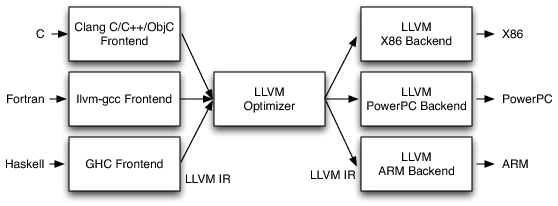
\includegraphics[width=0.8\textwidth]{LLVMCompiler1.png}
  \caption{процес компилације LLVM. Слика преузета са чланка \textit{LLVM - The archicture of open source applications}  }
  \label{fig:grafikon}
\end{figure}

\subsection{Предњи део компајлера}
 Предњи део компајлера задужен је за парсирање, валидацију и проналазак грешака у изворном
 к\^{o}ду, затим за превођење парсираног к\^{o}да у међурепрезентацију LLVM.
 Превођење се обично изводи, прво изградњом апстрактног синтаксног стабла (AST [5]), а затим  и превођењем AST-а у међурепрезентацију.
 У суштини сваки програмски језик, уколико имплементира предњи део који може да
 изгенерише међурепрезентацију LLVM, може користити алат за оптимизацију или 
 задњи део LLVM-а.
 Најбитнији пројекат који имплементира предњи део LLVM-a је Clang.
 Clang је предњи део компајлера за програмске језике  C, C++ и Objective C.


 \subsection{Алат за оптимизацију}
 Алат за оптимизацију (opt [6]) дизајниран је тако да на улазу прима LLVM
 међурепрезентацију и изврши оптимизације над међурепрезентацијом.
 Овај алат је организован у више низова оптимизационих пролаза, тако да је излаз
 једне оптимизације улаз у другу.
 Неки од примера оптимизационих пролаза су уметање, елиминација мртвог к\^{o}да,
 реалокација израза, размотавање петљи итд. 
 Од нивоа оптимизације зависе и оптимизациони пролази који ће бити покренути.
 У наставку ћемо приказати основне нивое оптимизације у случају Clang-a [28]\footnote{Наведени пролази алата за оптимизацију су везани за верзију 6.0 Clang-a}
 \begin{enumerate}
 \item O0 --  основне оптимизације, корисне због брзине компајлирања и лакшег
 			дебаговања.
 			Једна од опција које се задају алату за оптимизацију  на овом нивоу је
 			\texttt{-always-inline} (извршиће се уметање само оних функција које су експлицитно означене са always-inline).
 \item O1 -- додаје велики број пролаза у односу на ниво 0, неке од опција које
 			се задају алату за оптимизацију су:
           \texttt{-strip-dead-prototypes} (елиминација декларација функција за које не постоји имплементација), \texttt{-loop-rotate} (ротација петље), \texttt{-loop-deletion} (елиминација петљи чије извршавање не утиче на повратну вредност функције), \texttt{-loop-unroll} (одмотавање петље). 
           
 \item O2 -- овај ниво садржи све пролазе као ниво О1 уз додате опције: 
 \texttt{-inline} (уметање функције), \texttt{-gvn} (елиминација редундантних инструкција), -constmerge (спаја поновљене глобалне константе у једну заједничку).
 У овом нивоу се избацује опција \texttt{-always-inline} који ниво О0 додаје.
 \item O3 -- најећи ниво оптимизације, генерише извршни фајл који се најбрже извршава
 	али по цену времена компилације. Садржи пролазе као ниво О2 уз \texttt{-argpromotion} (функцијама које имају аргументе показивачког типа и уколико се само користи вредност
 	на коју реферише показивач, односно не мења се вредност у меморији, овај пролаз ће заменити показивачки тип са типом на који показује, када је то могуће).
 \end{enumerate}

\subsection{Задњи део компајлера} 
Задњи део LLVM-a генерише од међурепрезентације машински к\^{o}д за специфичну архитектуру. 
Главна компонента задњег дела је генератор к\^{o}да [7] (eng. LLVM code generator) који
користи сличан приступ као алат за оптимизацију, то јест дели генерисање машинског
к\^{o}дa на мање пролазе, који имају за циљ генерисање најбољег могућег к\^{o}да.
Најбитнији пролази су бирање инструкција, алокација регистара, распоређивање
(eng. scheduling).
LLVM може генерисати код за велики број архитектура, неке од њих су: x86, ARM,
PowerPC, SPARC.

\section{Предности LLVM-a}

Инфраструктура LLVM-а је бесплатна и њен изворни к\^{o}д је у потпуности доступан, 
што је навело не само истраживаче са универзитета, већ и велики број компанија 
да учествују у развоју, тако да данас значајан број људи активно 
учествује у одржавању и унапређивању овое инфраструктуре.
Модуларни дизајн омогућава лако мењање постојећих алата или додавање нових.
Захваљујући овом дизајну врло лако је додати нови предњи део компајлера, задњи део или
оптимизациони пролаз.
Такође, LLVM подржава и:
\begin{enumerate}
\item JIT компилацију [8]
\item оптимизацију током линковања (LTO [10])
\end{enumerate}

\chapter{Оптимизација целовитог програма}

Обично изворни к\^{o}д програма делимо у више компилационих јединица (eng. compilation unit) \footnote{често се назива и јединица превођења}.
Компајлер чита фајл по фајл и за сваки генерише њему одговарајући објектни фајл,
то јест свакој компилационој јединици одговара један објектни фајл.
Овако чинимо наш к\^{o}д читљивијим, омогућавамо паралелелно компајлирање више 
фајлова али и избегавамо потребу за компајлирањем целог програма за сваку промену
у узворном к\^{o}ду.
Овакав приступ има и лошу страну, пошто компајлер преводи фајл по фајл, он нема 
информације о к\^{o}ду који се налази у другим компилационим јединицама.
Због тога што компајлер не види тела функција имплементираних у другим компилационим
јединицама, не може у потпуности да сагледа логику и изврши жељене оптимизације.
Овај проблем се може решити уз помоћ линкера,
оптимизацијом током линковања (LTO) или спајањем свих фајлова у један и извршавањем
оптимизација на једном великом фајлу (eng. unity build [9]).

У наредном примеру биће показано због чега оптимизација целовитог програма 
може бити корисна.

\begin{lstlisting}[frame=single,caption={Пример позивања функције без тела}, captionpos=b]
//a.h                             //a.cpp
void do_nothing();                void do_nothing(){} 

//main.cpp          
#include "a.hpp"

int main(){
    for (int i = 0; i < 1'000'000'000; i++){
        do_nothing();
    }
}
\end{lstlisting}

У листингу 3.1  функција  \texttt{do{\_}nothing} има празно тело.
Уколико овај к\^{o}д преведемо са оптимизацијом -О3, без оптимизације целовитог програма, добићемо  резултат приказан у листингу 3.2:

\begin{lstlisting}[frame=single, caption={Резултат са оптимизацијом целовитог програма}, captionpos=b]
clang++  main.cpp a.cpp  -O3 -g
time ./a.out 
real    0m1,022s
user    0m1,014s
sys     0m0,000s
\end{lstlisting}

Може се приметити да је рачунару било потребно више од једне секунде да изврши програм који не ради ништа.
У наставку ћемо исте фајлове превести са оптимизацијом целовитог програма:
\begin{lstlisting}[frame=single, caption={Резултат без оптимизације целовитог програма}, captionpos=b]
clang++  main.cpp a.cpp  -O3 -flto=full -g
time ./a.out 
real    0m0,003s
user    0m0,003s
sys     0m0,000s
\end{lstlisting}

Разлика у времену извршавања је незанемарљива, као што се може видети у листингу 3.3.
У листингу 3.4 имамо приказ међурепрезентације LLVM  без и са укљученом оптмизацијом целовитог програма
и биће анализиране разлике између њих.
\begin{lstlisting}[frame=single, caption={Међурепрезентација без оптимизације целовитог програма}, captionpos=b]
; Function Attrs: norecurse uwtable
define i32 @main() local_unnamed_addr #0 !dbg !9 {
  call void @llvm.dbg.value(metadata i32 0, 
  metadata !14, metadata !DIExpression()), !dbg !16
  br label %2, !dbg !17

; <label>:1:                                  ; preds = %2
  ret i32 0, !dbg !18

; <label>:2:                                  ; preds = %2, %0
  %3 = phi i32 [ 0, %0 ], [ %4, %2 ]
  call void @llvm.dbg.value(metadata i32 %3, 
  metadata !14, metadata !DIExpression()), !dbg !16
  tail call void @_Z10do_nothingv(), !dbg !19
  %4 = add nuw nsw i32 %3, 1, !dbg !22
  call void @llvm.dbg.value(metadata i32 %4,
  metadata !14, metadata !DIExpression()), !dbg !16
  %5 = icmp eq i32 %4, 1000000000, !dbg !23
  br i1 %5, label %1, label %2, !dbg !17, !llvm.loop
}

; Function Attrs: nounwind readnone speculatable
declare void @llvm.dbg.value(metadata, metadata, metadata)

; Function Attrs: norecurse nounwind readnone uwtable
define void @_Z10do_nothingv() local_unnamed_addr #2 
 !dbg !26 {
  ret void, !dbg !29
}
\end{lstlisting}


\begin{lstlisting}[frame=single, caption={Међурепрезентација са оптимизацијом целовитог програма}, captionpos=b]
; Function Attrs: norecurse nounwind readnone uwtable
define dso_local i32 @main() local_unnamed_addr #0 
!dbg !9 {
  call void @llvm.dbg.value(metadata i32 0, 
  metadata !14, metadata !DIExpression()), !dbg !16
  ret i32 0, !dbg !17
}

; Function Attrs: nounwind readnone speculatable
declare void @llvm.dbg.value(metadata, metadata, metadata)

\end{lstlisting}

У листингу 3.4, где није укључена оптимизација целовитог програма, компајлер нема информацију  како
изгледа функција \texttt{do{\_}nothing} и компајлер генерише к\^{o}д који је у петљи милион пута позива.
У листингу 3.5, када је укључена оптимизација целовитог програма, компајлер има информацију о телу те функције,
упознат је са тим да она не ради ништа, тако да може да оптимизује не само позивање те функције,
односно да је уметне, већ може да уклони комплетну петљу, јер после уметања
функције \texttt{do{\_}nothing} тело петље остаје празно.
Видимо да је елиминисана и функција \texttt{do{\_}nothing} из извршног програма и да је унутар
функције \texttt{main} остало само враћање резултата.
О уметању и елиминацији мртвог к\^{o}да биће више речи у наставку.

Оптимизација целовитог програма се такође може користити за детекцију недефинисаног
понашања, када компајлер нема увид у цео к\^{o}д у јединици превођења и без
активне оптимизације целовитог програма компајлер не може програмеру да укаже
на грешку, чак и када су сва обавештења укључена (-Wall).
У компајлеру gcc је ова подршка имплементирана, што можемо видети у раду
\textit{Undefined behavior in theory and practice} [26], тако да се у будућности ова
функционалност очекује и у компајлеру clang.

\section{Ортимизација током линковања}


Захваљујући модуларном дизајну LLVM-a и чињеници да можемо компајлирати део к\^{o}да,
сачувати резултат и наставити компилацију касније без губитака информација
слику 2.1 можемо допунити додавањем линкера и оптимизацијама током процеса линковања.

\begin{figure}[!ht]
  \centering
  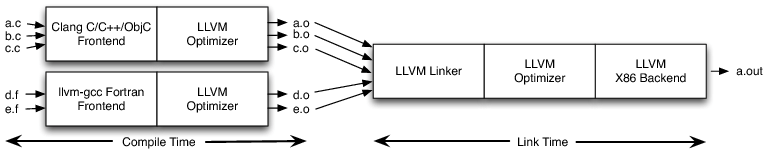
\includegraphics[width=0.8\textwidth]{LTO.png}
  \caption{LLVM процес компилације са подршком линкера. Слика преузета са чланка \textit{LLVM - The archicture of open source applications} }
  \label{fig:grafikon}
\end{figure}


У наставку ћемо објаснити због чега је линкер користан у оптимизацији целовитог програма.

Главни задатак линкера је да све објектне фајлове споји у један фајл, извршни фајл
или дељену библиотеку. 
Да би испунио овај задатак линкер прво мора да извши реалокацију симбола и резолуцију
симбола.
Симболи могу бити глобалне променљиве, функције, класе итд. 
Сваки објектни фајл садржи табелу симбола у којој се налазе сви симболи који 
могу бити дефинисани у истом објектном фајлу или у неком другом.
Уколико симбол није дефинисан унутар објектног фајла он ће у табели симбола бити
означен као "extern", у супротном биће означен као "import".
Да би се успешно превео програм у извршни фајл, линкер прво мора да пронађе све 
недостајуће симболе у свим објектним фајловима и повеже их са тачно једном дефиницијом, то јест да изврши резолуцију симбола.
Затим линкер траба да упише адресе симбола (такође задатак
линкера је да и неким импортованим симболима промени адресу, уколико је компајлер то назначио), односно да изврши реалокацију симбола.
Због ових својстава линкер има пресудну улогу у оптимизацији целовитог програма.
Линкер 
има увид у све табеле симбола и алат за оптимизацију може то искористити за оптимизације
делова к\^{o}да који су му пре били "невидљиви". 

У наставку приказаћемо интеракцију између линкера и алата за оптимизацију.
Оптимизација током линковања у инфраструктури LLVM садржи четири фазе:
\begin{enumerate}
\item Читање фајлова битк\^{o}д 
\item Резолуција симбола
\item Оптимизовање фајлова битк\^{o}д
\item Резолуција симбола након оптимизације
\end{enumerate}

\subsection{Читање фајлова битк\^{o}д}
Сви објектни фајлови долазе до линкера, који из њих чита и сакупља информације
о симболима, који су присутни у фајловима.
Ови фајлови могу бити у форми фајлова битк\^{o}д LLVM или стандардних објектних
фајлова (eng. native object files).
Линкер већ има могућност за третирање објектних фајлова.
Да би могао
правилно да чита и фајлове битк\^{o}д LLVM  потребна му је помоћ, а то му омогућава
 libLTO [11].
libLTO је библиотека који је намењена за коришћење од стране линкера.
libLTO има стабилан интерфејс, тако да је могуће користити
LLVM алат за оптимизацију, без потребе за излагањем интерног LLVM к\^{o}да.
Такође, још једна предност ове библиотеке је то што можемо мењати LLVM LTO к\^{o}д независно
од линкера, то јест не морамо за сваку промену к\^{o}да који имплементира
оптимизације мењати и линкер.

Уколико линкер добије
објектни фајл, он већ зна да чита тај фајл и додаће симболе у глобалну табелу симбола.
Уколико је у питању фајл  битк\^{o}д LLVM , линкер ће позвати функције \\
\texttt{lto{\_}module{\_}get{\_}symbol{\_}name} и 
\texttt{lto{\_}module{\_}get{\_}symbol{\_}attribute }
libLTO библиотеке да би добио све дефинисане  симболе, затим ће те симболе, 
као у случају стандардног објектног фајла, додати у глобалну табелу симбола.

\subsection{Резолуција симбола}
Као што је већ објашњено у фази читања фајлова битк\^{o}д, линкер покушава да разреши све симболе помоћу
глобалне табеле симбола.
Уколико је укључена опција елиминације мртвог к\^{o}да линкер чува листу симбола који
су коришћени у осталим објектним фајловима, такозвани живи симболи.
Опција елиминације мртвог к\^{o}да је подразумевано укључена
уколико се користи оптимизација током линковања.

\subsection{Оптимизација фајлова битк\^{o}д} 
У овој фази линкер користи информације из глобалне табеле симбола, и пријављује
живе симболе алату за оптимизацију функцијом \\
\texttt{lto{\_}codegen{\_}add{\_}must{\_}preserve{\_}symbol}.
Затим линкер позива алат за отимизацију и генератор к\^{o}да над фајловима битк\^{o}д
функцијом \texttt{lto{\_}codegen{\_}compile}, чији је резулат објектни фајл
који je настао спајањем више фајлова битк\^{o}д, са примењеним оптимизацијама на њима.
Примећујемо да је оптимизације могуће извршити искључиво на фајловима битк\^{o}д,
то јест објектни фајлови се не оптимизују на овај начин.

\subsection{Резолуција симбола након оптимизације}
У овој фази линкер чита оптимизоване објектне фајлове и ажурира табелу симбола уколико 
има неких промена. На пример уколико је укључена елиминација мртвог к\^{o}да,
линкер може да избаци неке симболе из табеле.
У овој фази нема више фајлова битк\^{o}д, то јест сви фајлови су објектни фајлови.
Након оптимизације наставља се са процесом изградње к\^{o}да као да оптимизације
није ни било.

\section{Оптимизација целовитог програма без подршке линкера}

Приступ отимизације целовитог програма са линкером захтева линкер Gold [12],
који у себи има подршку за библиотеку libLTO.
На неким системима овај линкер није доступан и ту је немогуће извршити стандардну
оптимизацију током линковања.
Алтернативни приступ је спајање свих фајлова битк\^{o}д LLVM  у један фајл битк\^{o}д
и извршавање оптимизација над тим фајлом.
Ово је могуће захваљујући LLVM-ов алату llvm-link [13].

Овим приступом добијамо исте перформансе као са приступом где имамо подршку линкера,
са тим што овај приступ неће радити уколико сви фајлови нису фајлови битк\^{o}д,
односно не ради са објектним фајловима.


\section{Уметање функција}

Уобичајена пракса у програмирању је издвајање к\^{o}да који се понавља у 
засебне функције.
Издвајање к\^{o}да је корисно зато што на тај начин избацујемо копирање
истог к\^{o}да на више места у програму.
На тај начин не само да се повећава читљивост програма, већ се смањује
могућност грешака, које су честе при копирању  к\^{o}да.
Са друге стране, позиви функција могу бити захтевни што се тиче времена извршавања.
Када се функција позове долази до креирања новог стек оквира, померања показивача
инструкција на почетак те функције, чувања тренутног стања позиваоца функције у 
регистрима и слично.
Такође,  к\^{o}д функције може бити ван кеша инструкција, што може битно
утицати на време извршавања програма.
Решење ових проблема је уметање функција [14] (eng. function inlining).
Уметање је замена позива функције у компајлираном к\^{o}ду
целокупним телом позване функције.
Поред тога што уметање елиминише утрошено време позива функције, оно такође
омогућава компајлеру да генерише оптималан к\^{o}д.
Пошто је цео к\^{o}д функције уметнут, компајлер може извршити оптимизације у већем
блоку, што некада може довести до значајних убрзања.
\par
Показано је да уметање функција може бити корисно и намеће се логично питање --
када је могуће извршити уметање?
Неке функције можемо одмах елиминисати из списка кандидата за уметање, уколико имамо дељену динамичку библиотеку, компајлер нема
информацију о к\^{o}ду функције тако да је не може уметнути.
Сличан проблем је са функцијама које се налазе у другим објектним фајловима.
\par 
Видели смо да уметање има велики број предности, али да га није могуће увек
урадити, да ли онда увек уметнути функцију када је то могуће?
Одговор је не. 
Поред великог броја предности, уметање има и неке мане.
Једна од мана је повећање величине извршног фајла, поготово када функције имају
велики број инструкција.
Због тога ипак мора постојати компромис између перфоманси програма и величине
извршног фајла.
\par
Функције са великим бројем инструкција могу негативно да утичу на перфомансе, тако
што утичу на кеш инструкција, јер велики број инструкција руши локалност референци. 
На пример уколико компајлер уметне функцију са великим бројем инструкција 
унутар петље, врло је могуће да тај блок више не стаје у кеш инструкција,
и онда при свакој итерацији петље долази до промашаја кеша. Због тога се
обично избегава уметање оваквих функција.
Такође, функције које се скоро никада не  позивају, нема смисла уметати.
Уметањем таквих функција нећемо добити никакве предности
у перфомансама, само можемо повећати величину извршног фајла.
\par
Да би компајлер генерисао оптмималан к\^{o}д, користи хеуристике, преко којих одређује
да ли неку функцију треба уметнути или не.
Битне информације које користе хеуристике су колико функција има инструкција,
колико пута се позива у току програма, да ли је функција коришћена у осталим
објектним фајловима и слично.
\par
Поред ове статичке анализе сложености функција, где користимо фиксиране границе (eng. threshold)
за број иснтрукција, позива итд. и тако одређујемо да ли треба да уметнемо функцију,
постоји и динамчка анализа.
Динамичка анализа користи информације које се добијају приликом профајлирања програма.
На овај начин можемо добити прецизније информације и самим тим боље перфомансе програма после оптимизације,
али само у случају да тестно окружење програма симулира реалну ситуацију у којој
ће се програм извршавати.
У супротном можемо добити лошије перфомансе него статичком анализом.
Профајлирањем можемо открити делове к\^{o}да који се чешће извршавају, и компајлер 
поклања посебну пажњу оптимизовању и уметању функција које се налазе у тим деловима.

Програмер може у изворном  к\^{o}ду сигнализирати компајлеру да изврши уметање
атрибутом \texttt {always{\_}inline}, на системима \texttt{Unix}, али ни то не гарантује да ће на крају
функција заиста бити уметнута.
\par
У наставку биће приказан један пример где је могуће извршити уметање уколико
је укључена оптимизација целовитог програма.

\begin{lstlisting}[frame=single,caption={Пример уметања функције}, captionpos=b]
//square.hpp           
int square(int);         
    					
//square.cpp				
int square(int a){
    return a *a;
}

//main.cpp
#include "square.hpp"
#include <iostream>

int main(){
    int result = 0;
    
    for (int i = 0; i < 100; i++){
        result+= square(i);
    }
    std::cout << result;
}

\end{lstlisting}

У наставку приказаћемо разлике међурепрезентације LLVM без и са оптимизације
целовитог програма. Преведен\footnote{сви примери у раду преведени су компајлером Clang са нивоом оптимизације -О3 и опцијом -g.} је к\^{o}д из листинга 3.6.

\begin{lstlisting}[frame=single,caption={Међурепрезентација без оптимизације целовитог програма}, captionpos=b]
 Function Attrs: norecurse uwtable
define i32 @main() local_unnamed_addr #4 !dbg !966 {
  call void @llvm.dbg.value(metadata i32 0, 
  metadata !968, metadata !DIExpression()), !dbg !971
  call void @llvm.dbg.value(metadata i32 0, 
  metadata !969, metadata !DIExpression()), !dbg !972
  br label %3, !dbg !973

; <label>:1:                              ; preds = %3
  %2 = tail call dereferenceable(272) 
  %"class.std::basic_ostream"* 
  @_ZNSolsEi(%"class.std::basic_ostream"* 
  nonnull @_ZSt4cout, i32 %7), !dbg !974
  ret i32 0, !dbg !975

; <label>:3:                              ; preds = %3, %0
  %4 = phi i32 [ 0, %0 ], [ %8, %3 ]
  %5 = phi i32 [ 0, %0 ], [ %7, %3 ]
  call void @llvm.dbg.value(metadata i32 %5, 
  metadata !968, metadata !DIExpression()), !dbg !971
  call void @llvm.dbg.value(metadata i32 %4, 
  metadata !969, metadata !DIExpression()), !dbg !972
  %6 = tail call i32 @_Z6squarei(i32 %4), !dbg !976
  %7 = add nsw i32 %6, %5, !dbg !979
  %8 = add nuw nsw i32 %4, 1, !dbg !980
  call void @llvm.dbg.value(metadata i32 %8, 
  metadata !969, metadata !DIExpression()), !dbg !972
  call void @llvm.dbg.value(metadata i32 %7, 
  metadata !968, metadata !DIExpression()), !dbg !971
  %9 = icmp eq i32 %8, 100, !dbg !981
  br i1 %9, label %1, label %3, !dbg !973, !llvm.loop !982
}

; Function Attrs: nounwind readnone speculatable
declare void @llvm.dbg.value(metadata, 
metadata, metadata) #5

declare dereferenceable(272)
 %"class.std::basic_ostream"* 
 @_ZNSolsEi(%"class.std::basic_ostream"*, i32) 
 local_unnamed_addr #1

; Function Attrs: nounwind readnone uwtable
define i32 @_Z6squarei(i32) local_unnamed_addr
 #6 !dbg !984 {
  call void @llvm.dbg.value(metadata i32 %0, 
  metadata !986, metadata !DIExpression()), !dbg !987
  %2 = mul nsw i32 %0, %0, !dbg !988
  ret i32 %2, !dbg !989
}
\end{lstlisting}

\begin{lstlisting}[frame=single,caption={Међурепрезентација са оптимизацијом целовитог програма}, captionpos=b]
; Function Attrs: norecurse uwtable
define dso_local i32 @main() local_unnamed_addr 
#4 !dbg !966 {
  call void @llvm.dbg.value(metadata i32 0, 
  metadata !968, metadata !DIExpression()), !dbg !971
  call void @llvm.dbg.value(metadata i32 0, 
  metadata !969, metadata !DIExpression()), !dbg !972
  %1 = tail call dereferenceable(272) 
  %"class.std::basic_ostream"* 
  @_ZNSolsEi(%"class.std::basic_ostream"* nonnull 
  @_ZSt4cout, i32 328350), !dbg !973
  ret i32 0, !dbg !974
}

; Function Attrs: nounwind readnone speculatable
declare void @llvm.dbg.value(metadata,
 metadata, metadata) #5

declare dereferenceable(272) 
%"class.std::basic_ostream"* 
@_ZNSolsEi(%"class.std::basic_ostream"*, i32) 
local_unnamed_addr #1

\end{lstlisting}

Ако погледамо међурепрезентацију из листинга 3.7, без оптимизације целовитог програма, видимо да је она јако
слична изворном к\^{o}ду, компајлер не види тело функције \texttt{square}, тако да не може неке 
значајније оптимизације да изврши.
Са друге стране у листингу 3.8, када је укључена оптимизација целовитог програма, компајлер
успева да уметне функцију.
Овим се компајлер не само да генерише  к\^{o}д који не садржи трошак позива функција, већ омогућава и остале оптимизације.
Зато што сада имамо тело функције у блоку петље, компајлер увиђа да се петља извршава константан
број пута и да нема потребе стално израчунавати исту приликом покретања програма, већ вредност
променљиве result може да се израчуна у току компилације програма, самим тим се компајлер елиминише петљу и к\^{o}д око ње.
У позиву  функције видимо резултат израчунавања :
\begin{lstlisting}[frame=single]
tail call dereferenceable(272) %"class.std::basic_ostream"*
@_ZNSolsEi(%"class.std::basic_ostream"
* nonnull @_ZSt4cout, i32 328350)
\end{lstlisting}
Такође, више нема потребе за постојањем функције \texttt{square} (више се нигде не користи)
и она је избрисана из извршног фајла.



\section{Елиминација мртвог к\^{o}да}

Елиминација мртвог к\^{o}да [16] (eng. dead code elimination) је компајлерска 
оптимизација која елиминише к\^{o}д који не утиче на резултат извршавања
програма.
Уклањање мртвог к\^{o}да има многе предности: смањује величину извршног програма,
побољшава локалност инструкција, уклањањем непотребних инструкција такође
повећава брзину извршавања програма.
Без укључене оптимизације целовитог програма компајлер може да елинише локалне
променљиве, уметнуте статичке функције као и статичке глобалне променљиве.
То ради једноставним праћењем позива свих статичких глобала и сврставањем истих
у живе или мртве скупове, у зависности да ли се глобал користи или не.
Глобали су идентификатори који имају глобални опсег (еng. scope).
То значи да су они видљиви унутар целог програма, то јест свака јединица превођења
може видети глобал дефинисан у некој другој јединици превођења.
Због тога сме постојати само једна дефиниција глобала.
Глобали могу бити функције, променљиве, класе...
Све глобале из мртвог скупа, на крају оптимизационих пролаза, можемо елиминисати.
Са укљученом оптимизацијом целовитог програма можемо избацити не само статичке
глобалне променљиве или функције, него све глобале који се не користе.
Овај поступак се извршава током линковања и описан је у секцији  3.1.

Пример елиминације мртвог к\^{o}да смо већ видели у листингу 3.8
у којем је компајлер уклонио функцију \texttt{square} јер се није користила. Програм
у листингу 3.9 приказаће ово на неколико очигледнијих примера:

\begin{lstlisting}[frame=single,caption={Пример елиминације мртвог к\^{o}да}, captionpos=b]
//a.hpp
int foo1(void);
void foo2(void);
void foo4(void);

//a.cpp
#include "a.hpp"

static signed int i = 0;

void foo2(void) {
  i = -1;
}

static int foo3() {
  foo4();
  return 10;
}

int foo1(void) {
  int data = 0;

  if (i < 0)
    data = foo3();

  data = data + 42;
  return data;
}

//main.cpp
#include <iostream>
#include "a.hpp"

void foo4(void) {
  std::cout << ("Hi\n");
}

int main() {
  return foo1();
}

\end{lstlisting}

\begin{lstlisting}[frame=single,caption={Међурепрезентација без оптимизације целовитог програма}, captionpos=b]
 Function Attrs: uwtable

declare dereferenceable(272) 
%"class.std::basic_ostream"* @_ZSt16__
ostream_insertIcSt11char_traitsIcEERSt13basic_
ostreamIT_T0_ES6_PKS3_l
(%"class.std::basic_ostream"* 
dereferenceable(272), i8*, i64) local_unnamed_addr #1

; Function Attrs: uwtable
define void @_Z4foo4v() local_unnamed_addr #0 !dbg !983 {
  call void @llvm.dbg.value(metadata 
  %"class.std::basic_ostream"* @_ZSt4cout, 
  metadata !984, metadata !DIExpression()), !dbg !1048
  call void @llvm.dbg.value(metadata i8* 
  getelementptr inbounds ([4 x i8], [4 x i8]*
   @.str, i64 0, i64 0), 
  metadata !993, metadata !DIExpression()), !dbg !1050
  %1 = tail call dereferenceable(272) 
  %"class.std::basic_ostream"*
   @_ZSt16__ostream_insertIcSt11char_
  traitsIcEERSt13basic_ostreamIT_T0_ES6_PKS3_l
  (%"class.std::basic_ostream"* nonnull dereferenceable(272) 
  @_ZSt4cout, i8* nonnull getelementptr 
  inbounds ([4 x i8], [4 x i8]* @.str, i64 0, i64 0), 
  i64 3), !dbg !1051
  ret void, !dbg !1053
}

; Function Attrs: norecurse uwtable
define i32 @main() local_unnamed_addr #5 !dbg !1054 {
  %1 = tail call i32 @_Z4foo1v(), !dbg !1055
  ret i32 %1, !dbg !1056
}

; Function Attrs: norecurse nounwind uwtable
define void @_Z4foo2v() local_unnamed_addr #6 !dbg !1057 {
  store i1 true, i1* @_ZL1i, align 4
  ret void, !dbg !1058
}

; Function Attrs: uwtable
define i32 @_Z4foo1v() local_unnamed_addr #0 !dbg !1059 {
  call void @llvm.dbg.value(metadata i32 0,
   metadata !1061, metadata !DIExpression()), !dbg !1062
  %1 = load i1, i1* @_ZL1i, align 4
  br i1 %1, label %2, label %3, !dbg !1063

; <label>:2:                              ; preds = %0
  tail call void @_Z4foo4v(), !dbg !1064
  call void @llvm.dbg.value(metadata i32 10, 
  metadata !1061, metadata !DIExpression()), !dbg !1062
  br label %3, !dbg !1068

; <label>:3:                              ; preds = %2, %0
  %4 = phi i32 [ 52, %2 ], [ 42, %0 ]
  call void @llvm.dbg.value(metadata i32 %4, 
  metadata !1061, metadata !DIExpression()), !dbg !1062
  ret i32 %4, !dbg !1069
}

\end{lstlisting}


\begin{lstlisting}[frame=single,caption={Међурепрезентација са оптимизацијом целовитог програма }, captionpos=b]
; Function Attrs: norecurse nounwind readnone uwtable
define dso_local i32 @main() local_unnamed_addr #4 
!dbg !982 {
  ret i32 42, !dbg !983
}
\end{lstlisting}

У листингу 3.10, без оптимизације целовитог програма, видимо да је компајлер уметнуо
функцију \texttt{foo3} и она се не налази унутар извршног фајла.
Компајлер је успео да елиминише функцију јер је она статичка, али остале нису
тако да се оне налазе у извршном фајлу.
Видимо да је и к\^{o}д међурепрезентације сличан изворном, тако да компајлер поред
уметања, није успео да изврши неке веће оптимизације.

Са друге стране, у листингу 3.11, са оптимизацијом целовитог програма, видимо да је у
извршном фајлу остала само функција \texttt{main}, која враћа вредност 42.
Да бисмо утврдили како се то догодило, пролази се кроз цео процес оптимизације овог 
програма, са укљученом оптимизацијом целовитог програма.
\par
Линкер прво препознаје да се функција \texttt{foo2} не користи нигде у програму, шаље ту
информацију компајлеру (конкретно алату за оптимизацију) и он је брише.
Чим обрише функцију, алат за оптимизацију види да услов \texttt{i < 0} никада није испуњен,
тако да може да обрише и тај део к\^{o}да али и функцију \texttt{foo3}, јер се она сада
више неће користити.
Линкер сада препознаје да се функција \texttt{foo4} не користи више тако да се и она брише.
На крају остаје само функција \texttt{foo1} која увек враћа вредност 42, то алат за оптимизацију
препознаје, уметне је, брише и враћа вредност 42 као повратну вредност функције
\texttt{main}.

\section{Девиртуализација}
 Девиртуализација [17] (eng. devirtualization) је поступак замене виртуалних позива
 функција непосредним позивима.
 Виртуални позиви функција су спорији од непосредних, што у системима
 у којима је брзина извршавања програма кључна може да буде велики проблем.
 Због тога је пожељно извршити девиртуализацију кад год је то могуће.
 Девиртуализација се најефикасније може извршити приликом оптимизације целовитог
 програма, али постоје три случаја у којима компајлер може да закључи да је 
 девиртуализација могућа, без увида у целокупан програмски к\^{o}д.
 Прво ће бити описани ти случајеви.
 
 \subsection{Познат динамички тип објекта}
 Уколико је компајлеру познат динамички тип објекта при компајлирању, он може 
 да девиртуализује позив функције.
 
 \begin{lstlisting}[frame=single,caption={Пример са познатим динамичким типом објекта }, captionpos=b]
#include <iostream>
struct Base{
    virtual int f(){return 1;}
};

struct Derived : Base{
    int f() override {return 2;}
};

int main(){
    Derived d;
    Base * b = new Base();
    std::cout << b->f();
    std::cout << d.f();  
}
 \end{lstlisting}
 
 \begin{lstlisting}[frame=single,caption={Међурепрезентација програма из листинга 3.12}, captionpos=b]
; Function Attrs: norecurse uwtable
define i32 @main() local_unnamed_addr #4 !dbg !964 {
  call void @llvm.dbg.value(metadata %struct.Derived* undef,
   metadata !966, metadata !DIExpression()), !dbg !985
  %1 = tail call dereferenceable(272) 
  %"class.std::basic_ostream"* @_ZNSolsEi
  (%"class.std::basic_ostream"* nonnull @_ZSt4cout, i32 1), 
  !dbg !986
  call void @llvm.dbg.value(metadata %struct.Derived* undef, 
  metadata !966, metadata !DIExpression()), !dbg !985
  %2 = tail call dereferenceable(272) 
  %"class.std::basic_ostream"* @_ZNSolsEi
  (%"class.std::basic_ostream"* nonnull @_ZSt4cout, 
  i32 2), !dbg !987
  ret i32 0, !dbg !988
}
 \end{lstlisting}
 
 У листингу 3.13 види се да компајлер успешно девиртуализује и умеће позив 
 \texttt{f->b()} јер има информацију да је променљива \texttt{b} иницијализована на 
 \texttt{new Base()}.
 Променљива \texttt{d} је типа \texttt{Derived}, па ту и не постоји виртуелни позив
  и поред тога што је чланска функција \texttt{f} виртуална.
 \footnote{Када променљива није показивачког или референцног типа 
  компајлер зна да позив не може бити виртуалан.}
 
 \subsection{Кључна реч final}
 У програмском језику C++ kључна реч \texttt{final} означава да функција не може бити 
 преправљена (eng. override) у изведеној класи (уколико се кључна реч \texttt{final} налази у потпису функције)
 или да се из те класе не може извести нова класа (уколико се кључна реч \texttt{final}
 налази у потпису класе).
	 
\begin{lstlisting}[frame=single,caption={Пример са кључном речју final }, captionpos=b]
struct Base{
    virtual int f(){return 1;}
};

struct Derived final : Base{
    int f() override {return 2;}
};
int func(Derived *d){
    return d->f();
}

\end{lstlisting}
 
 За разлику од примера у листингу 3.12 овде смо структуру \texttt{Derived} обележили кључном 
 речју \texttt{final}.
 То говори компајлеру да ни у овој, али ни у било којој другој јединици превођења, 
 не може постојати структура која је изведена из структуре \texttt{Derived}.
 То сазнање омогућава компајлеру да изврши девиртуализацију позива функције \texttt{f()}.
 Примећујемо када не бисмо експлицитно обележили  Derived са \texttt{final} девиртуализација
 не би била могућа, јер компајлер не може да зна да ли у некој другој јединици превођења
 постоји структура изведена из структуре \texttt{Derived} и самим тим преправљена функција.
 
 \subsection{Унутрашња видљивост}
 Када кажемо да нека променљива или функција има унутрашњу видљивост [18]
 (eng. internal linkage) то значи да је она видљива само унутар своје јединице
 транслације.
 Што значи да уколико имамо структуру, или класу, која има унутрашњу видљивост,
 комапјлер може девиртуализовати позив функције јер је сигуран да она неће моћи бити
 преправљена.
 Овај принцип је сличан додавању кључне речи  \texttt{final}.
 Један једноставан начин да класа добије унутрашњу видљивост јесте смештање исте
 у безимени простор имена [19] (eng. unnamed namespace).
 Овај принцип приказан је у листингу 3.15.
 
 \begin{lstlisting}[frame=single,caption={Пример са унутрашњом видљивости}, captionpos=b]
namespace{
struct Base{
    virtual int f(){return 1;}
};

struct Derived : Base{
    int f() override {return 2;}
};
}
\end{lstlisting}
 
\subsection{Девиртуализација помоћу оптимизације целовитог програма}
 
 Приказане су ситуације када компајлер без оптимизације целовитог програма може да
 изврши девиртуализацију.
 У већини ситуација нећемо наилазити на тако једноставне случајеве, а и често ће
 дефиниције виртуалних функција бити у другим јединицама транслације.
 Због тога што компајлер види цео програм, када је укључена оптимизација
 целовитог програма, он види и функције и класе, тако да може да изврши
 девиртуализацију агресивније.
 У наставку биће приказан  пример у листингу 3.16, који има само један изворни фајл и 
 његове одговарајуће међурепрезентације у листинзима 3.17 и 3.18.
 \begin{lstlisting}[frame=single,caption={Пример девиртуализације}, captionpos=b]
#include <iostream>
struct Base
{
  virtual int f() { return 1; }
};

struct Derived : public Base
{
  int f() override { return 2; }
};

int g(Derived *obj)
{
  return obj->f();
}

int main()
{
  Derived *obj = new Derived();
  std::cout << g(obj);
}
\end{lstlisting}
	
\begin{lstlisting}[frame=single,caption={Међурепрезентација без оптимизације целовитог програма }, captionpos=b]
; Function Attrs: uwtable
define i32 @_Z1gP7Derived(%struct.Derived*)
 local_unnamed_addr #0 !dbg !964 {
  call void @llvm.dbg.value(metadata %struct.Derived* %0,
   metadata !985, metadata !DIExpression()), !dbg !986
  %2 = bitcast %struct.Derived* %0 to i32 
  (%struct.Derived*)***, !dbg !987
  %3 = load i32 (%struct.Derived*)**, 
  i32 (%struct.Derived*)*** %2, 
  align 8, !dbg !987, !tbaa !988
  %4 = load i32 (%struct.Derived*)*, 
  i32 (%struct.Derived*)** %3, 
  align 8, !dbg !987
  %5 = tail call i32 %4(%struct.Derived* %0), !dbg !987
  ret i32 %5, !dbg !991
}

; Function Attrs: nounwind readnone speculatable
declare void @llvm.dbg.value(metadata,
 metadata, metadata) #4

; Function Attrs: norecurse uwtable
define i32 @main() local_unnamed_addr #5 
!dbg !992 {
  %1 = tail call dereferenceable(272) 
  %"class.std::basic_ostream"* 
  @_ZNSolsEi(%"class.std::basic_ostream"* nonnull 
  @_ZSt4cout, i32 2), !dbg !995
  ret i32 0, !dbg !996
}
\end{lstlisting}

\begin{lstlisting}[frame=single,caption={Међурепрезентација са оптимизацијом целовитог програма }, captionpos=b]
; Function Attrs: norecurse uwtable
define dso_local i32 @main() local_unnamed_addr #4 !dbg !964 {
  %1 = tail call dereferenceable(272) 
  %"class.std::basic_ostream"* 
  @_ZNSolsEi(%"class.std::basic_ostream"* nonnull
   @_ZSt4cout, i32 2), !dbg !984
  ret i32 0, !dbg !985
}
\end{lstlisting}

У листингу 3.17 постоје инструкције за узимање вредности
виртуалног показивача и позивање виртуалне функције, што значи да компајлер није успео
да девиртуализује позив иако види тело функције и класе.
То се дешава због тога што компајлер не зна да ли у некој другој јединици превођења
постоји класа која је изведена из класе \texttt{Derived} и због тога не може да изврши
оптимизације.
Са укљученом оптимизацијом целовитог програма компајлер види да не постоји класа
изведена из класе \texttt{Derived} и компајлер успешно девиртуализује, а затим и умеће
позив функције. 
 
 \chapter{ThinLTO}
 
 У претходном поглављу описане су оптимизације које омогућава оптимизација целовитог програма и које могу  значајно
 побољшати перформансе нашег програма.
 Такође, видели смо како је имплементирана стандардна оптимизација током линковања,
  линкер добија фајлове битк\^{o}д, уместо објектних фајлова, затим се ти
фајлови битк\^{o}д спајају у један и над тим фајлом се врше све оптимизације.
 
\begin{figure}[!ht]
  \centering
  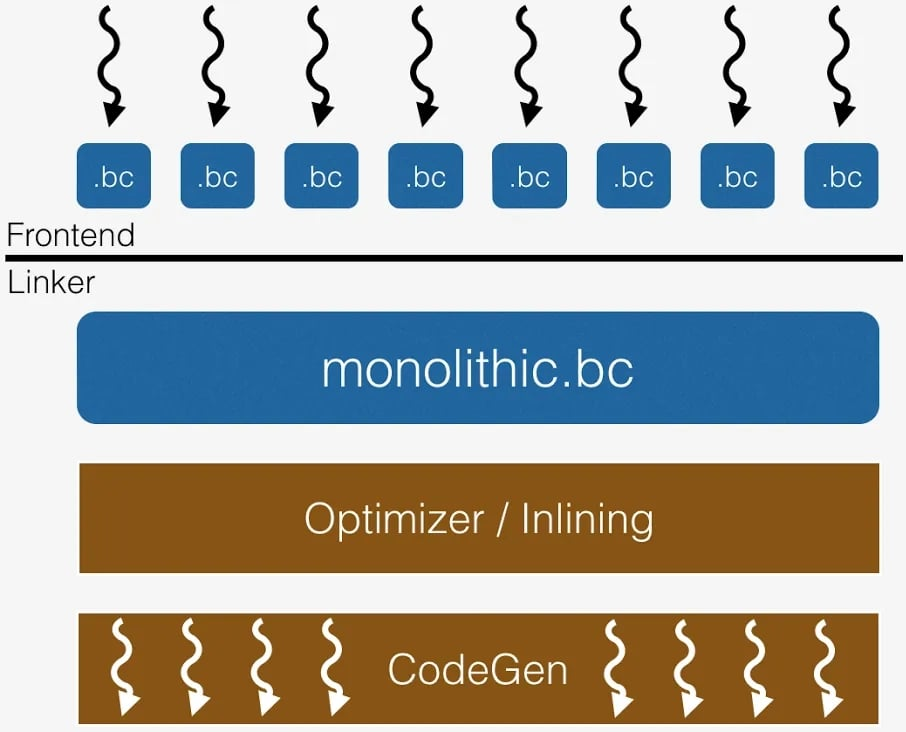
\includegraphics[width=0.8\textwidth]{LTO_normal.png}
  \caption{Стандардни процес оптимизације током линковања. Сликa преузетa са чланка \textit{"ThinLTO: Scalable and Incremental LTO"} [21]}
  \label{fig:grafikon}
\end{figure}

Стандардни приступ има неколико мана.
Први проблем је то што се губи предност паралелног компајлирања, која постоји 
када није активна оптимизација целовитог програма.
На слици 4.1 се види да постоји паралелно превођење изворних фајлова у 
фајлове битк\^{o}д али због спајања свих фајлова у један велики фајл битк\^{o}д,
та предност се касније губи зато што све оптимизације над тим фајлом морају 
да се раде без могућности парелелизације.
Због тога компајлирање траје много дуже него без оптимизације целовитог програма.
Такође, за сваку промену у било ком изворном фајлу, морају се испочетка
вршити све оптимизације на обједињеном фајлу, што поново изузетно утиче не време
превођења.
Још један велики проблем овог приступа је то што сада у меморији морају да се налазе  међурепрезентације свих компилационих јединица одједном, спојене
у једну. 
Често је немогуће извршити оптимизацију целовитог програма, поготово на 
машинама које немају велику радну меморију.
Приступ за решавање ових проблема је  ThinLTO [20].
\par ThinLTO је нови приступ који омогућава сличне перфомансе при превођењу
као када није укључена оптимизација целовитог програма, док задржава већину
оптимизација и самим тим перформансе извршног фајла као регуларна оптимизација
целовитог програма.
При оптимизацији ThinLTO, за разлику од класичне оптимизације целовитог програма, уместо учитавања фајлова битк\^{o}д и спајања у један,
ThinLTO за сваку јединицу превођења чува кратак
резиме за анализу у кораку линковања. 
Уз резиме чувају се и локације функција за касније уметање у друге јединице 
превођења.
Кључна оптимизација коју ThinLTO омогућава је убацивање само оних функција које
су потребне конкретном фајлу битк\^{o}д и које ће бити уметнуте у том фајлу битк\^{o}д.
И тај поступак се ради за сваки фајл битк\^{o}д, што значи да нема спајања, већ се и
даље поступак  извршава паралелно.
Процес оптимизације целовитог програма ThinLTO подељен је на три фазе:
\begin{enumerate}
\item Превођење -- генеришу се међурепрезензације као и у случају стандардног процеса
	оптимизације целовитог програма, са тим што сада имамо и резиме уз сваку
	међурепрезентацију.
\item Линковање -- линкер комбинује резимее из прошлог корака и врши анализу.
\item Задњи део -- паралелна оптимизација и генерисање к\^{o}да.
\end{enumerate}
 
\begin{figure}[!ht]
  \centering
  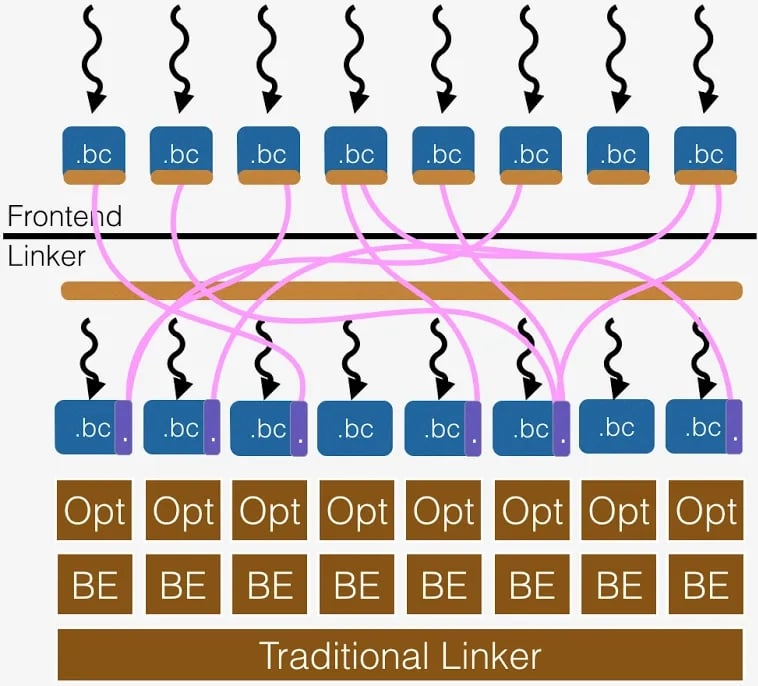
\includegraphics[width=0.8\textwidth]{LTO_thin.png}
  \caption{ThinLTO процес оптимизације. Сликa преузетa са чланка \textit{"ThinLTO: Scalable and Incremental LTO"}}
  \label{fig:grafikon}
\end{figure}

Кључни део оптимизације ThinLTO дешава се у првој фази, а то су креирања резимеа.
Свака глобална променљива и функција се налазе у резимеу, за ту јединицу превођења.
Резиме садржи по једно поље за сваки симбол и у том пољу
се налазе подаци који описују тај симбол.
На пример, за функцију, у пољу унутар резимеа може да стоји њена видљивост, 
број инструкција које функција садржи, информације за профајлирање уколико су потребне
и слично.
Додатно, свака референца према другом симболу (позив друге функције, узимање адресе,
приступање глобалу) се записује у резиме и тако се гради граф позива (eng. call graph).
Ове информације омогућавају креирање комплетног графа током фазе линковања.
ThinLTO је једноставно активирати, само је потребно додати  \texttt{-flto=thin} у командној линији
приликом компајлирања.

У наставку биће приказана разлиау између перформанси, меморијских захтева као и времена
компајлирања између оптимизације током линковања и ThinLTO-а.

\begin{figure}[!ht]
  \centering
  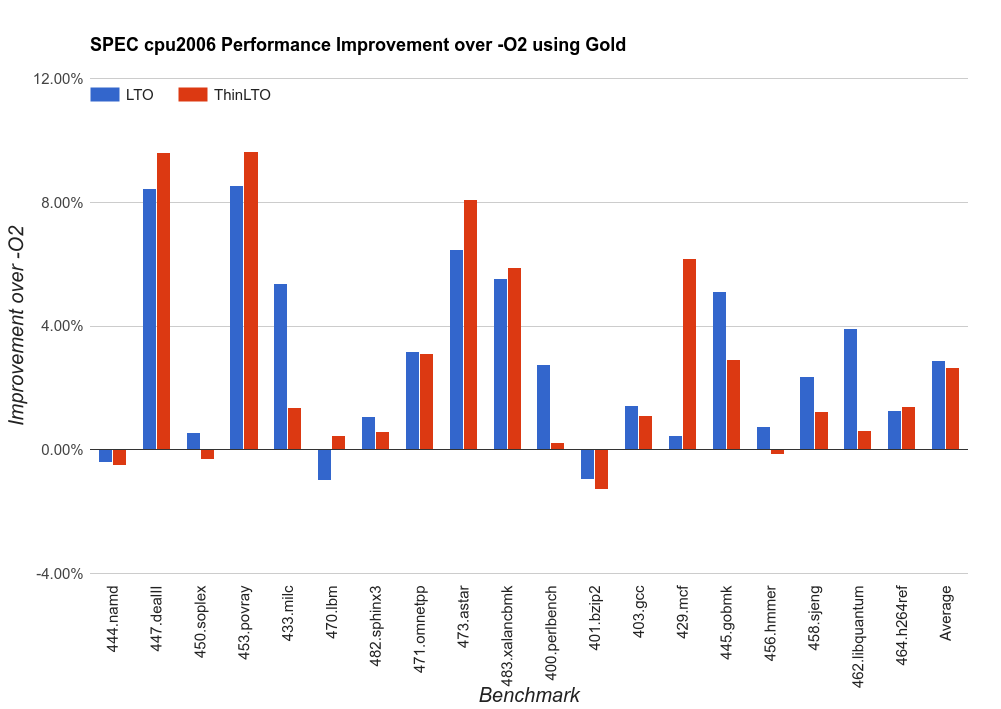
\includegraphics[width=0.8\textwidth]{thin_perfomance.png}
  \caption{Разлика у перформансама између ThinLTO и регуларне оптимизације током линковања. Сликa преузетa са чланка \textit{"ThinLTO: Scalable and Incremental LTO"}}
 
  \label{fig:grafikon}
\end{figure}

На слици 4.3 показано је да у просеку стандардна оптимизација даје за нијансу
боље резултате, али постоје ситуације када ThinLTO надмашује стандардну оптимизацију.


\begin{figure}[!ht]
  \centering
  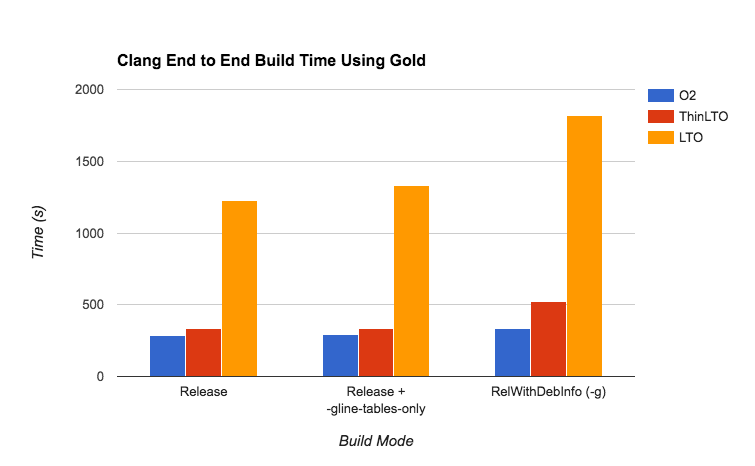
\includegraphics[width=0.8\textwidth]{build_time.png}
  \caption{Разлика у времену превођења програма
   између ThinLTO и регуларне оптимизације током линковања. Сликa преузетa са чланка \textit{"ThinLTO: Scalable and Incremental LTO"}}
  \label{fig:grafikon}
\end{figure}

На слици 4.4 види се да је време компајлирања програма са оптимизацијом ThinLTO
јако слично времену превођења без оптимизације током линковања.
Осетнија разлика између ова два начина компајлирања је приликом компајлирања
програма који има информације потребне за дебаговање, али у току су унапређења
у овом пољу, па се очекује смањење ове разлике у будућности.
Што се тиче регуларне оптимизације током линковања, компајлирање програма
је далеко спорије него код ThinLTO-а у сваком измереном случају.
 

\chapter{Алат за визуализацију промена}

Алат, \textit{compiler explorer LTO}, имплементиран као део овог рада визуализује
промене унутар међурепрезентације LLVM програма 
преведеног са и без оптимизације целовитог програма.
Инспирација за овај алат био је \textit{compiler explorer} [22].
Идеја креатора \textit{compiler explorerа} била је приказивање одговарајућих асемблерских
инструкција за сваку линију изворног к\^{o}да.
Ова функционалност је корисна јер програмер тако има увид у к\^{o}д који је 
компајлер изгенерисао за њега и евентуално може да пронађе неку грешку у 
изворном к\^{o}ду која је видљива тек након оптимизација, или да провери, колико је компајлер добро оптимизовао к\^{o}д након превођења.
Касније, је у \textit{compiler explorer} додата подршка и за приказ међурепрезентације LLVM 
јер је она разумљивија од конкретног асемблерског језика и садржи више опција
за дебаговање.
\textit{Compiler explorer} приказује промене у контексту једне јединице превођења,
 што значи да к\^{o}д мора да се успешно компајлира, али не мора да се линкује. 
 
Са друге стране, \textit{compiler explorer LTO}, 
приказује разлике у међурепрезентацијама које одговарају извршним фајловима који су
добијени компилацијом 
са и без укључене оптимизације целовитог програма.
За разлику од \textit{compiler explorer-а} за коришћење овог алата неопходно је да сви
улазни фајлови буду успешно линковани.
Због тога што су објектни фајлови линковани у извршни фајл, \textit{compiler explorer LTO} може да прикаже 
међурепрезентације извршних фајлова.
Алат повезује линије изворног к\^{o}да са одговарајућим линијама у међурепрезентацији LLVM, одговарајуће линије су приказане истом бојом.
Такође, постоји опција приказивања \textit{diff-a} [24] између међурепрезентација са и без
активне оптимизације целовитог програма.
Тренутно су подржани искључиво програми писани у програмском језику C++.
Изворни  к\^{o}д алата може се наћи на адреси [23].

Захтеви за покретање алата:
\begin{enumerate}
\item оперативни систем Linux -- за алате wllvm и kompare
\item python3
\item python3-tk -- за графички интерфејс
\item clang -- за превођење програма
\item llvm-dis [27] --  који врши конверзију из формата битк\^{o}д у
			читљиви формат
\item wllvm -- за добијање међурепрезентације из извршног фајла
\item kompare -- за графички приказ \textit{diff} фајла
\end{enumerate}

\begin{lstlisting}[frame=single,caption=Шаблон покретања алата,captionpos=b]
python3 main.py -i {putanja_do_foldera_sa_.cpp_fajlovima}
-o {nivo_optimizacije('0', '1', '2', '3', '4',
                     'z', 'g', 'z', 'fast)}

\end{lstlisting}

Алат је написан у програмском језику Python и садржи две главне функционалности.

Прва функционалност је приказ међурепрезентације LLVM са и без активне оптимизације
целовитог програма као и њихово мапирање са линијама у изворном к\^{o}ду.
Мапирање је имплементирано тако да једној линији у изворном к\^{o}ду придружује
одговарајуће линије у међурепрезентацијама.
Свако мапирање је обојено различитом бојом и обојене су само оне линије у изворном
к\^{o}ду које су се после свих оптимизација превеле у одговарајућу међурепрезентацију
 (линије које су избачене се не боје).
 
Изворни фајлови преводе се на два начина.

\begin{lstlisting}[frame=single, caption=Шаблон превођења изворних фајлова са оптимизацијом целовитог програма, captionpos=b]
clang++ {source_files} -O{optimization_level} -g -flto -Wl,-plugin-opt=save-temps
\end{lstlisting}
 
\begin{lstlisting}[frame=single, caption=Шаблон превођења изворних фајлова без оптимизације целовитог програма, captionpos=b]
wllvm++ -O{optimization_level} -g {source_files}
\end{lstlisting}
 
У листингу 5.2 опција \texttt{flto} покреће оптимизацију целовитог програма,
док опција \texttt{-plugin-opt=save-temps} чува привремене фајлове који настају
при компајлирању.
Ова опција је потребна да би алат \texttt{llvm-dis} извршио конверзију формата битк\^{o}д,
који одговара извршном фајлу, у читљиви формат.

У листингу 5.3 алат wllvm, који за превођење користи компајлер Clang, додаје унутар извршног фајла и формат битк\^{o}д. 
Командом \texttt{extract-bc} врши се вађење формата битк\^{o}д из извршног фајла, а затим се врши конверзија у читљиви формат, исто као у случају са оптимизацијом
целовитог програма.

Опција -g додаје дебаг информације унутар међурепрезентација.
Ове информације омогућавају повезивање изворног к\^{o}да и међурерпрезентације.
Поред инструкције LLVM, за коју постоји дебаг информација, додата је кључна реч
\texttt{!dbg} поред које стоји број.
\begin{lstlisting}[frame=single, caption=Пример debug кључне речи, captionpos=b]
  %4 = mul nsw i32 %0, %0, !dbg !974
\end{lstlisting}
Унутар међурепрезентације можемо наћи линију текста која даје више информација о
инструкцијама, то јест повезује их са изворним фајлом.
За повезивање кључан је број који се налази после \texttt{!dbg}.
\begin{lstlisting}[frame=single, caption=Пример debug линије која повезује изворни к\^{o}д са међурепрезентацијом, captionpos=b]
!974 = !DILocation(line: 8, column: 18, scope: !975)
\end{lstlisting}

Из листинга 5.5 види се да инструкција из листинга 5.4 одговара линији 8 изворног фајла.
\textit{Scope} даје информацију о опсегу дате инструкције.
Рекурзивним праћењем \textit{scope-a} долази се до конкретног изворног фајла, коме линија припада.

Друга функционалност је приказивање графичког \textit{diff-a} унутар алата kompare [25].
\textit{Diff} је алат за поређење садржаја два фајла.
Овај алат креира \textit{diff} фајл који представља разлике између улазних фајлова.
Постоји више формата \textit{diff} фајла. 
Тренутно најкоришћенији формат је \textit{unified} формат.
\textit{Diff} фајл се може креирати и без алата \textit{diff}.
Помоћу ове функционалности лако можемо видети који LLVM блокови су склоњени, 
промењени или додати.

Описано је добијање међурепрезентације од улазних фајлова.
У наставку приказаће се креирање \textit{diff} фајла од међуререпрезентација.
Повезивање линија између више различитих фајова извршено је енкодирањем "име фајла:линија изворног  к\^{o}да:LLVMIR".
Име фајла је обавезно да би направили разлику између истих линија  к\^{o}да у две различите јединице транслације.
При креирању \textit{diff} фајла занемарени су:
\begin{enumerate}
\item имена променљивих -- током компилације имена променљивих које компајлер генерише унутар међурепрезентације нису стабилна, па су изостављана приликом
креирања \textit{diff} фајлa; 
\item линије к\^{o}да које служе за дебаг информације (!dbg број). Бројеви у два
	фајла не морају бити исти, а утичу на \textit{diff} (слично као имена променљивих);
\item коментари.
\end{enumerate}

Наглашено је да енкодиране линије користимо за креирање \textit{diff} фајла.
Уколико након завршетка алгоритма између неке две линије нема разлике, онда ту
енкодирану линију задржавамо у \textit{diff} фајлу и приказујемо на излазу.
У супротном, приказаћемо линије које одговарају неенкодираним верзијама.
То јест, заменићемо у фајлу енкодиране линије њиховим правим вредностима у међурепрезентацијама.
На слици 5.4 на 55. линији види се пример енкодирања. 
Види се да је та линија из фајла \texttt{main.cpp} и да је то десета линија у том фајлу.
Та линија је иста у обе верзије (без активне и оптимизације целовитог програма
и са активном оптимизацијом целовитог програма).
Док на пример енкодиране линије 59 и 46 нису исте, па су приказане њихове
 одговарајуће неенкодиране линије. 

У наставку биће приказан рад алата над фајловима из листинга 5.6, 5.7 и 5.8.

\begin{lstlisting}[frame=single, caption=a.hpp, captionpos=b]
int calculate(int num);
\end{lstlisting}

\begin{lstlisting}[frame=single, caption=a.cpp, captionpos=b]
#include "a.hpp"

int g_i = 1;

int calculate(int a){
    if (g_i){
        return a * a;
    }
    else{
       return a + a;
    }  
}
\end{lstlisting}

\begin{lstlisting}[frame=single, caption=main.cpp, captionpos=b]
#include "a.hpp"
#include <iostream>

int main(){
    int n;
    std::cin >> n;
    
    int result = 0;

    for (int i = 0 ; i < n; i++){
        result += calculate(i);
    }

    return result;
}

\end{lstlisting}

Покретањем алата, добијамо следећу слику 5.1:

\begin{figure}[!ht]
  \centering
  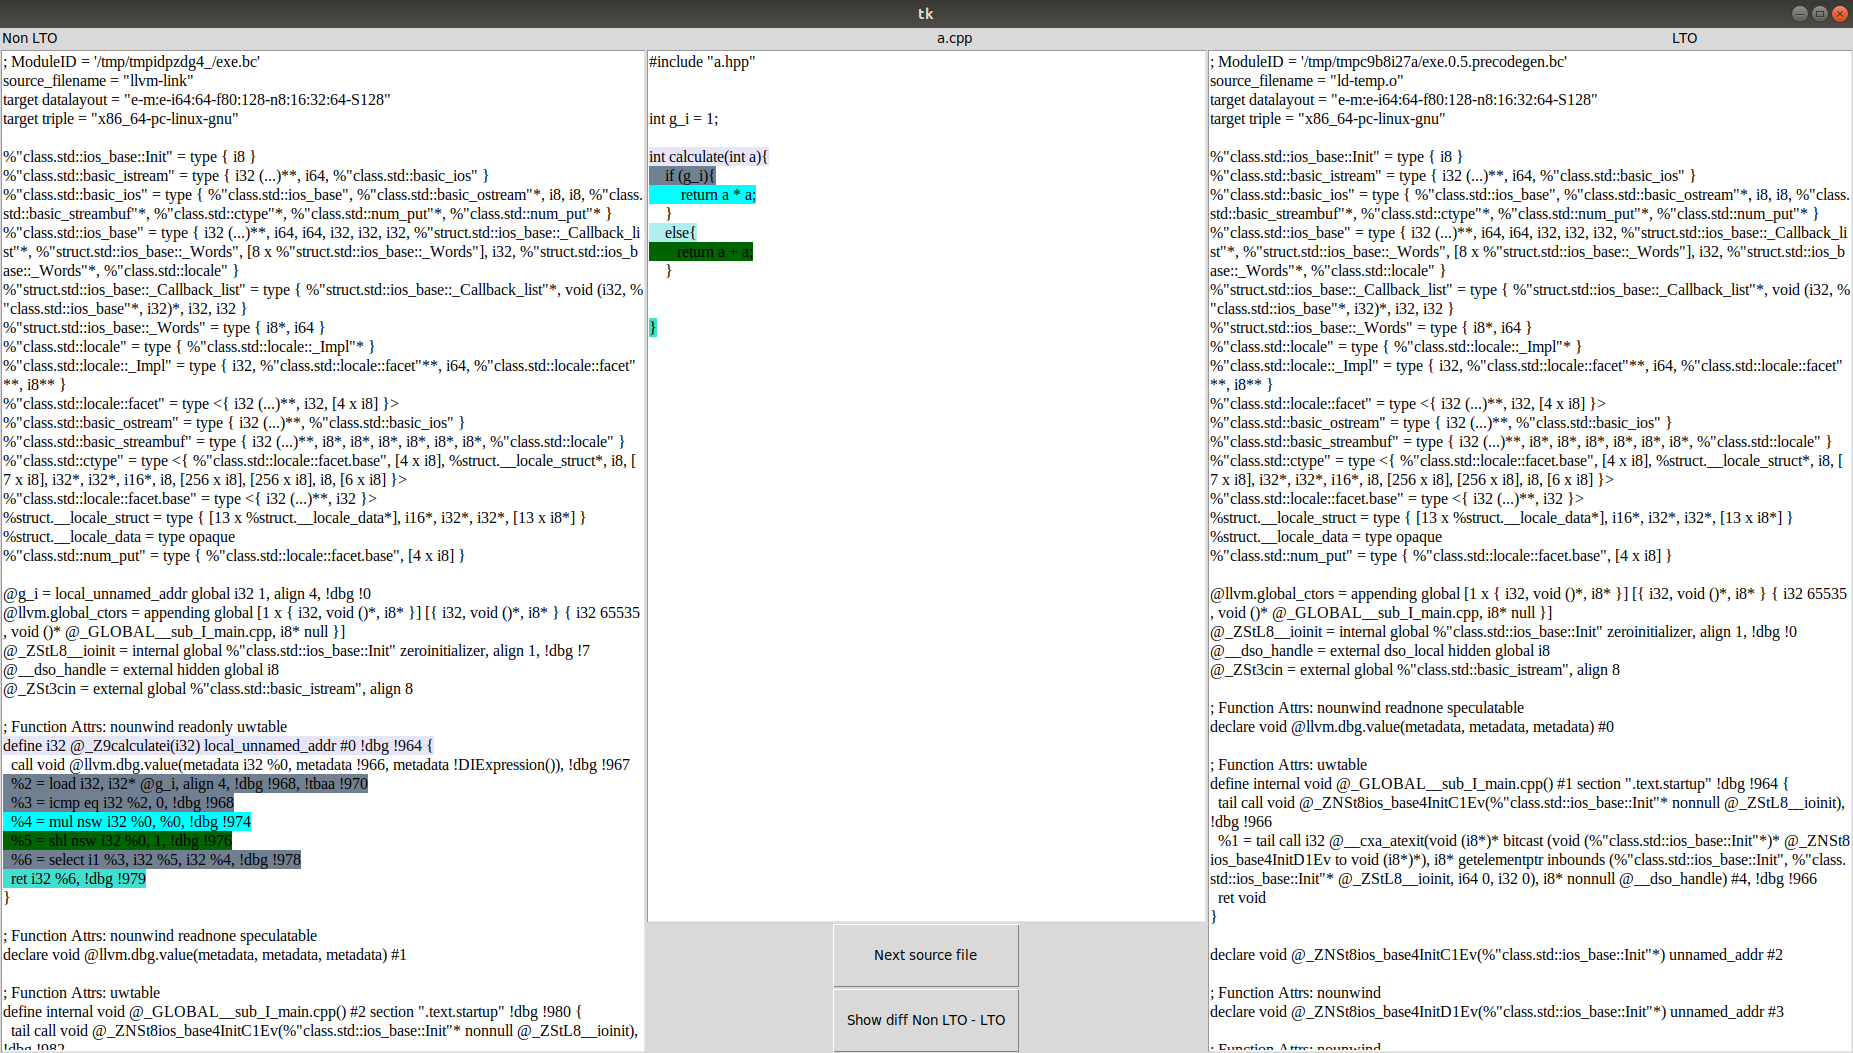
\includegraphics[width=0.8\textwidth]{a_cpp.png}
  \caption{ Повезивање линија изворног к\^{o}да и међурепрезентације у фајлу \textit{а.cpp }  }
  \label{fig:grafikon}
\end{figure}

У средњем прозору види се да је тренутни изворни фајл, који повезујемо са одговарајућим
међурепрезензацијама, фајл \texttt{a.cpp}.
Са његове леве стране налази се прозор међурепрезентације где није извршена оптимизација
целовитог програма, и обојене истим бојама одговарајуће линије у изворном и
фајлу LLVM.
Са десне стране се налази прозор са оптимизованом међурепрезентацијом где видимо
да ништа није обојено.
То је зато што је цео к\^{o}д  \texttt{a.cpp} фајла оптимизован
и не налази се у извршном фајлу.

Кликом на дугме \texttt{Next source file}, приказује се main.cpp фајл и одговарајуће 
мапирање линија.
\begin{figure}[!ht]
  \centering
  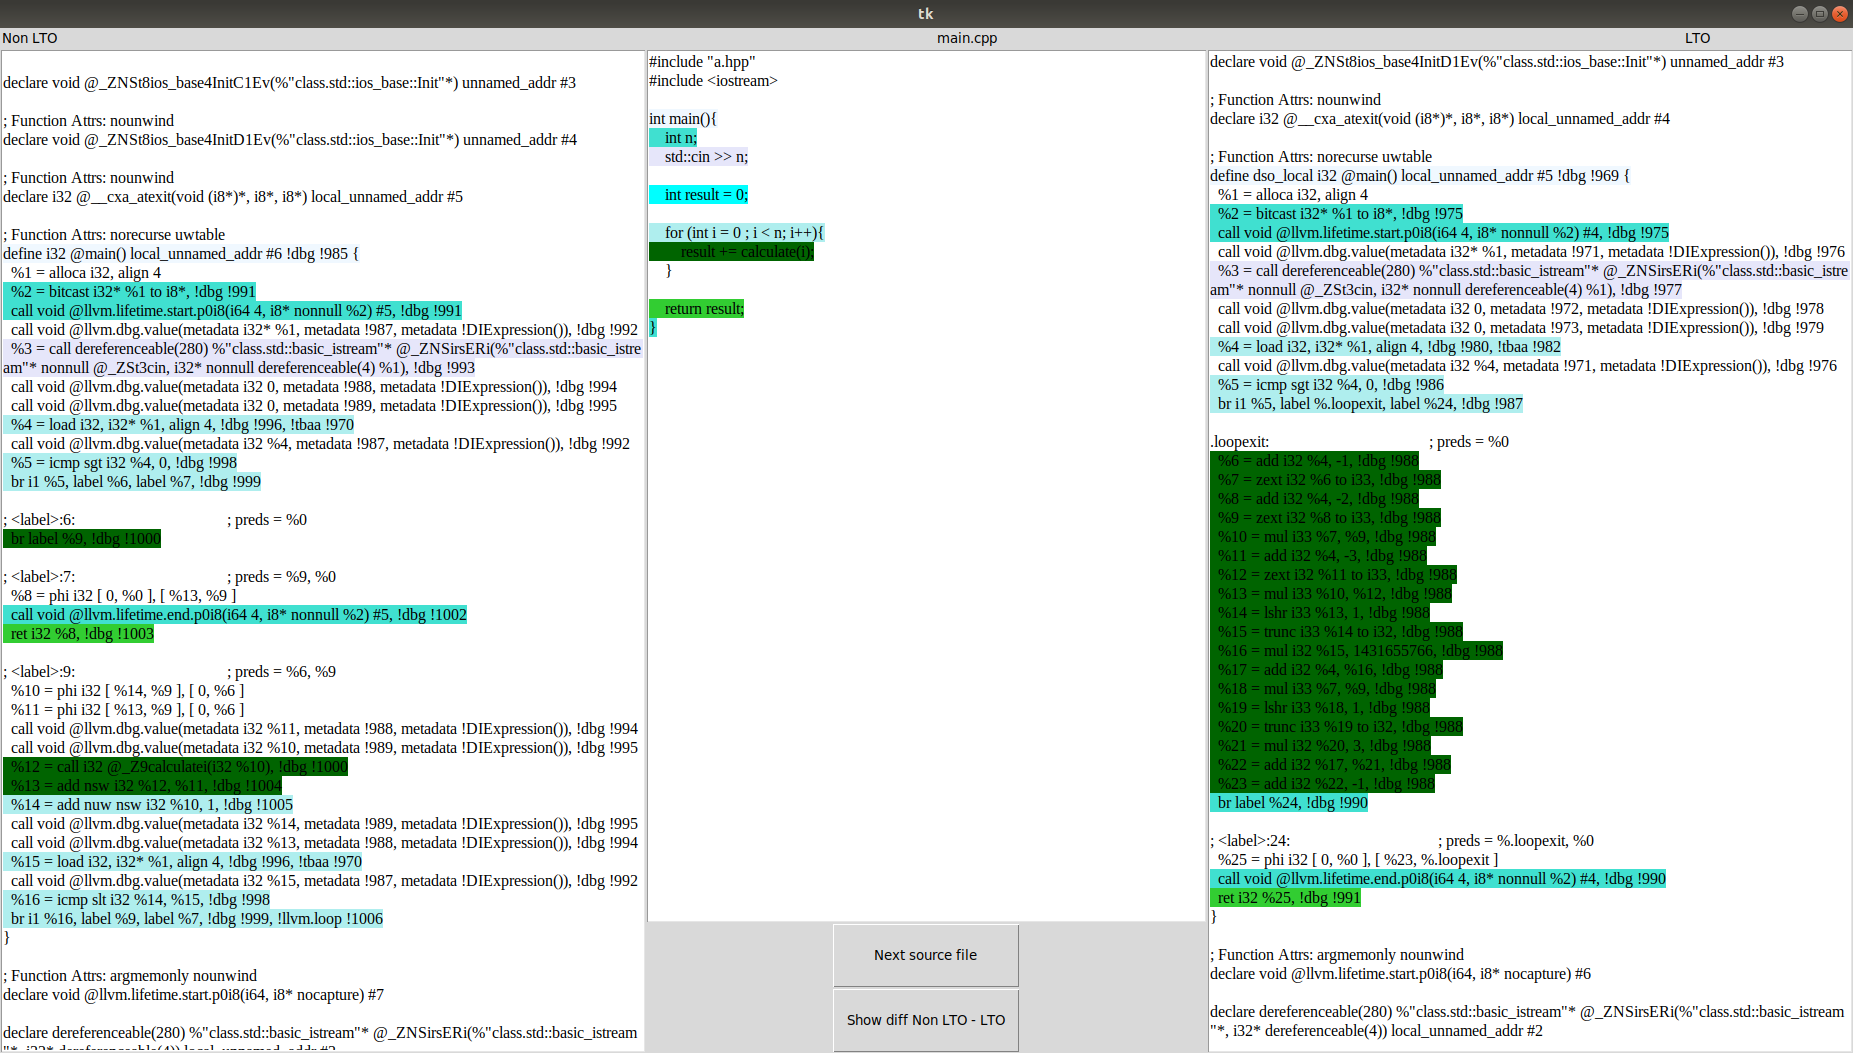
\includegraphics[width=0.8\textwidth]{main_cpp.png}
  \caption{Повезивање линија изворног к\^{o}да и међурепрезентације у фајлу \textit{main.cpp } }
  \label{fig:grafikon}
\end{figure}
Наравно, више се не приказују мапирања из претходног изворног фајла, већ само из
тренутног.

Кликом на дугме \texttt{Show diff} добија се приказ разлика између неоптимизоване и оптимизоване
верзије, приказане у алату kompare.
\begin{figure}[!ht]
  \centering
  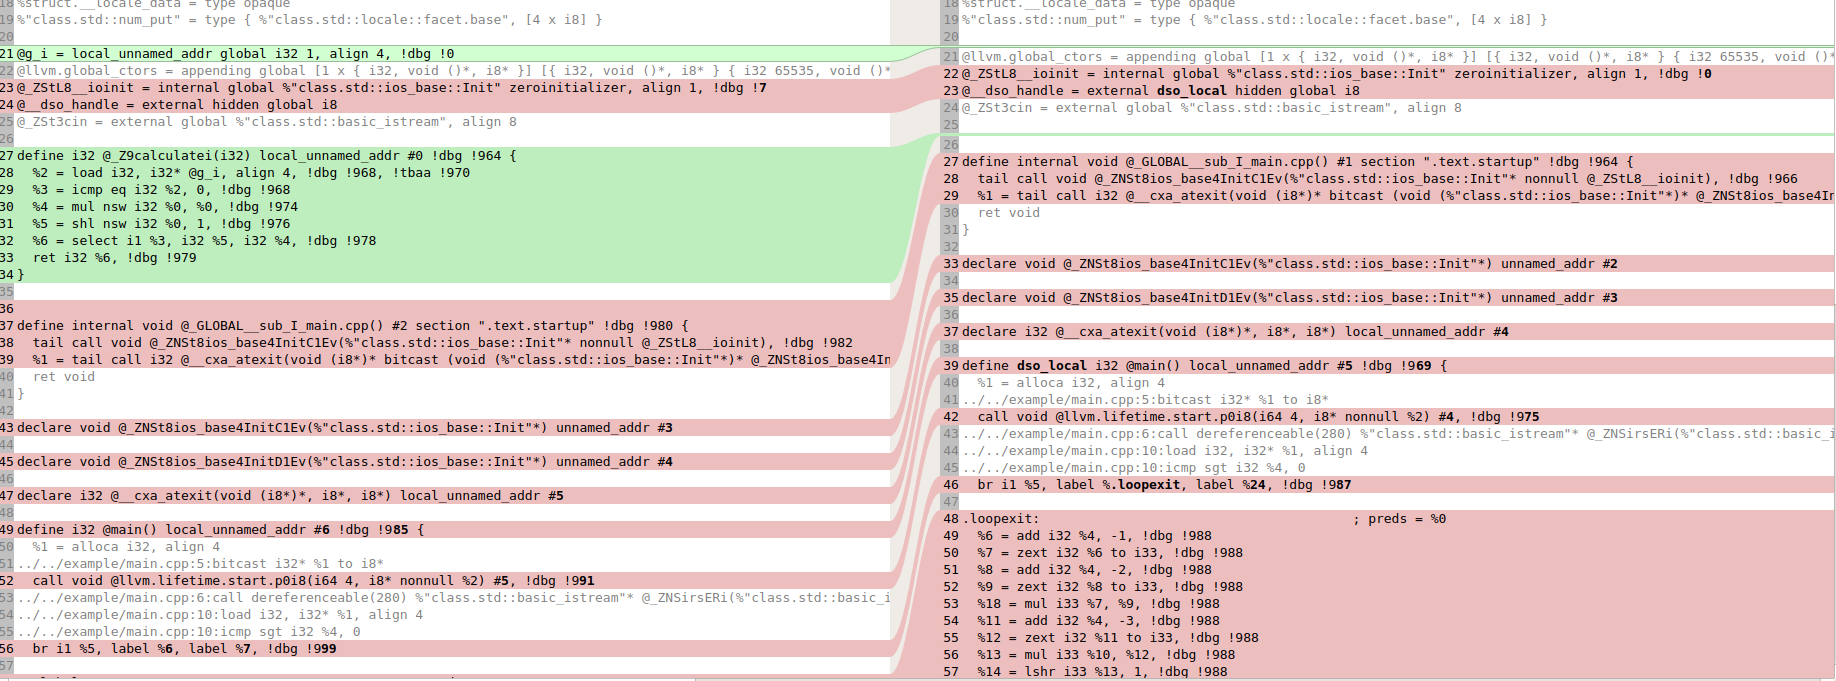
\includegraphics[width=0.8\textwidth]{diff_1.png}
  \caption{Први део \textit{diff} приказа неоптимизоване и оптимизоване верзије }
  \label{fig:grafikon}
\end{figure}
\begin{figure}[!ht]
  \centering
  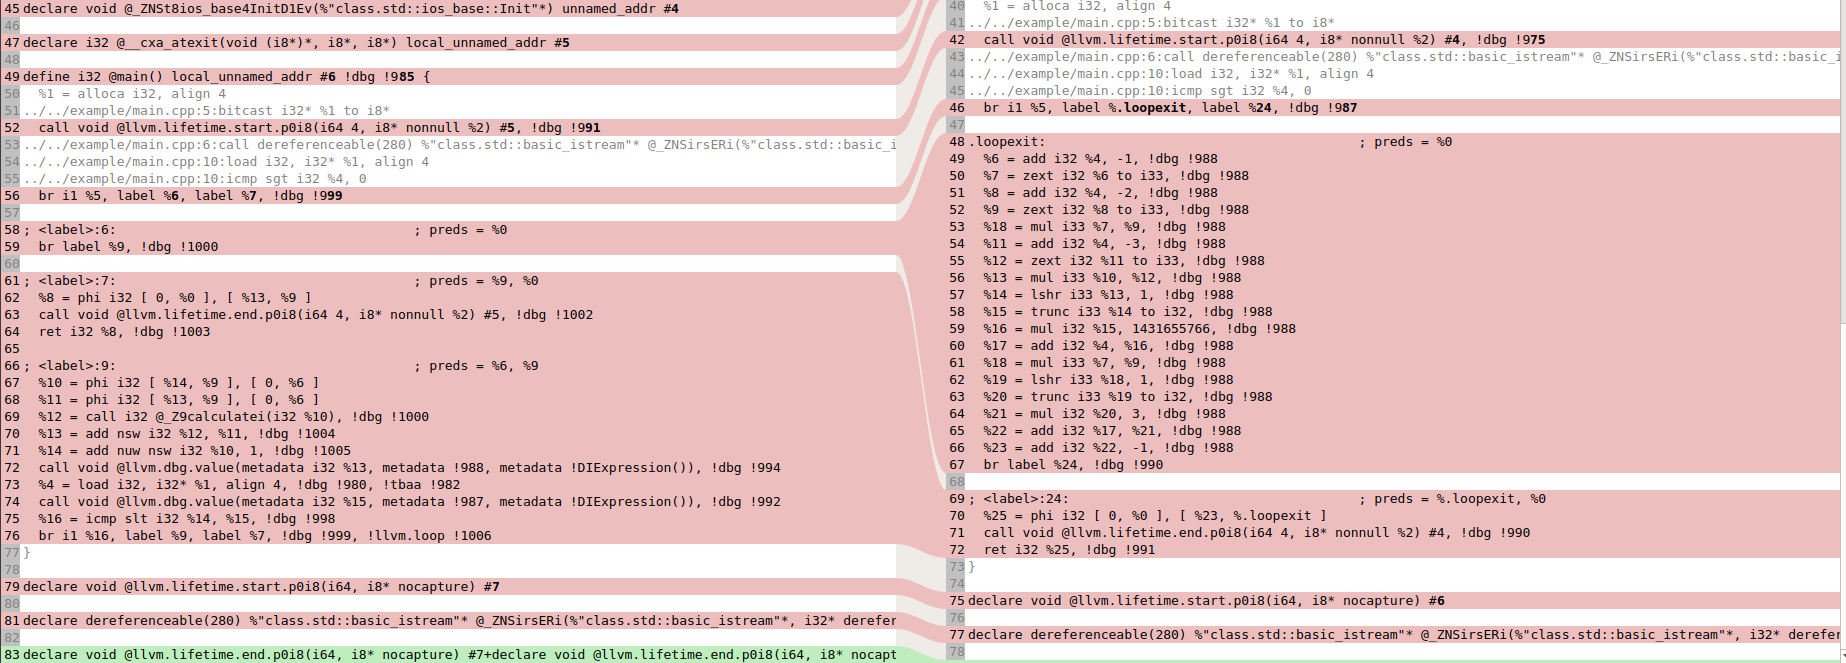
\includegraphics[width=0.8\textwidth]{diff_2.png}
  \caption{Други део \textit{diff} приказа неоптимизоване и оптимизоване верзије}
  \label{fig:grafikon}
\end{figure}

У примеру 5.1 видимо да је са активном оптимизацијом целовитог програма,
елиминисана глобална променљива g{\_}i  као и функција \texttt{calculate}.
Затим видимо и разлике у функцији \texttt{main}. 
Због тога што не види тело функције у верзији без активне оптимизације целовитог
програма, компајлер генерише к\^{o}д који позива функцију \texttt{calculate}.
У верзији са активном оптимизацијом целовитог програма, видимо не само да је функција
\texttt{calculate} уметнута, већ је избрисан део функције који никада није доступан
јер је вредност глобалне променљиве увек 1, а то се може видети тек после процеса
линковања.
Taкође, види се да је због уметања извршена и оптимизација петље.
Алат за
оптимизацију има информацију о телу \texttt{calculate} функције, помоћу тога он
закључује да се у петљи врши израчунавање збира квадрата првих n бројева.
Због те информације ово израчунавање може да се изврши без петље, математичком
формулом.
Петља је избачена и добијено је побољшање перформанси, јер нема потребе да се 
врти n пута.
% ------------------------------------------------------------------------------
\chapter{Закључак}
% ------------------------------------------------------------------------------
У раду је представљена компајлерска инфраструктура LLVM са посебним акцентом
на оптимизацију целовитог програма.
Видели смо да оптимизација целовитог програма доноси нека значајна побољшања
што се тиче времена извршавања и смањивања величине извршног фајла, али уз спорију
компилацију програма и већим заузећем меморије током тог процеса.
Ови проблеми су донекле решени новим приступом у оптимизацији целовитог програма
ThinLTO, али уз нешто лошије перформансе добијеног извршног фајла.
У будућности LLVM заједница ће активно наставити на решавању проблема код 
оба приступа.
\par
Као део рада имплементиран је алат који визуализује промене између
међурепрезентација преведених са и без активне оптимизације целовитог програма.
Алат омогућава програмеру да види које оптимизације је компајлер успео да изврши
тек након укључене оптимизације целовитог програма.
Ово је посебно корисно у едукативне сврхе као и за програмере који раде на самим
компајлерима, да би проверили како оптимизације раде и евентуално пронађу грешку
у имплементацијама неких оптимизација.



% ==============================================================================
% Završni deo teze i prilozi
\backmatter
% ==============================================================================
\chapter{Литература}
[1] LLVM Compiler Infrastructure -- https://llvm.org/docs/index.html \\

[2] LLVM Language Reference Manual -- https://llvm.org/docs/LangRef.html \\

[3] Appel, A., {\&} Ginsburg, M. (1997). Static Single-Assignment Form. 
     In Modern Compiler Implementation in C (pp. 433-473).  
   Cambridge: Cambridge University Press. doi:10.1017/CBO9781139174930.020 \\
 
[4] RISC --  Berezinski, John. "RISC — Reduced instruction set computer". Department of Computer Science, Northern Illinois University.  \\

[5] Abstract Syntax tree -- 
Harper, R. (2016). Abstract Syntax. In Practical Foundations for Programming Languages (pp. 3-11). Cambridge: Cambridge University Press. doi:10.1017/CBO9781316576892.003
\\

[6] Optimizer -- https://llvm.org/docs/CommandGuide/opt.html \\

[7] LLVM Code Generator -- https://llvm.org/docs/CodeGenerator.html \\

[8] Just In Time Compilation  -- Languages, Compilers, and Runtime Systems, University of Michigan, Computer Science and Engineering. \\

[9] Unity build -- https://onqtam.com/programming/2018-07-07-unity-builds/ \\ 

[10] Link Time Optimization -- https://llvm.org/docs/LinkTimeOptimization.html \\

[11] libLTO -- https://llvm.org/docs/LinkTimeOptimization.html{\#}liblto \\

[12] Gold linker -- https://llvm.org/docs/GoldPlugin.html \\

[13] llvm-link -- https://llvm.org/docs/CommandGuide/llvm-link.html \\

[14] Function inlining -- https://www.cs.cornell.edu/courses/cs6120/2019fa/blog/llvm-function-inlining/ \\

[15] The Architecture of Open Source Applications --https://www.aosabook.org/en/llvm.html \\

[16] Dead code elimination -- https://www.ibm.com/docs/en/adfz/developer-for-zos/14.0.0?topic=code-effects-dead-elimination \\

[17] Devirtualization -- https://blog.llvm.org/2017/03/devirtualization-in-llvm-and-clang.html \\

[18] Internal linkage -- https://www.learncpp.com/cpp-tutorial/internal-linkage/ \\

[19] Unnamed namespace -- https://www.ibm.com/docs/en/i/7.3?topic=only-unnamed-namespaces-c \\

[20] ThinLTO -- https://clang.llvm.org/docs/ThinLTO.html \\

[21] http://blog.llvm.org/2016/06/thinlto-scalable-and-incremental-lto.html \\

[22] https://godbolt.org/ \\

[23] https://github.com/filipl41/master \\

[24] Diff -- MacKenzie et al. "Binary Files and Forcing Text Comparison" in Comparing and Merging Files with GNU Diff and Patch. Downloaded 28 April 2007.\\

[25] Kompare -- https://apps.kde.org/kompare/ \\

[26] Undefined behavior in theory and practice -- https://queue.acm.org/detail.cfm?id=3468263 \\

[27] -- https://llvm.org/docs/CommandGuide/llvm-dis.html \\

[28] Clang optimization levels -- https://stackoverflow.com/questions/15548023/clang-optimization-levels

\end{document}